\chapter{Technical report}
%\chapter{Application à la Transmission d’un fichier quelconque (*.mpeg, *.mp3, *.txt, *.doc, *.pdf, etc)}

%\minitoc


\section{Guide on Eigenface prototype}
In this section, we will explain the implementation of  eigenface  method  with the differents expressions used to program
\paragraph{}
Using mostly PCA (Principal Components Analysis), eigenfaces method is based on the calculation of eigenvectors and eigenvalues.
The algorithm consists of two steps:
 \begin{itemize}
 \item the learning phase : in which the protoype define a projection space with several person images; 
 \item and the identification phase  : which consist in projecting the face of the person one needs to recognize from the database.
\end{itemize} 
 Those steps are presented as followed :
\subsection{Learning phase}
 The learning phase can be divided into several steps:
 \begin{itemize}
 \item Step 1 : It is necessary to have an image database containing M images taken in good conditions. In our case we used the  \href{http://www.cl.cam.ac.uk/Research/DTG/attarchive:pub/data/att_faces.zip}{AT\&T picture database} contains 400 images. The database includes 40 subjects and each subject has 10 differents images of himself so that he can be easily recognised in differents conditions (with glasses, a hat, a smiling face for instance...). All these images are the basis for learning. Each image is a matrix.
 \item Step 2 :Each image matrix is converted into vector.










\parbox{0.60\linewidth}{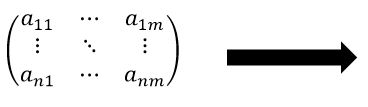
\includegraphics[scale=0.75]{matrice2vector}%[height=70mm,width=70mm]
}
\parbox{0.15\linewidth}{


%\begin{figure}[bth]%[!ht]
%\begin{center}
%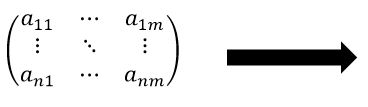
\includegraphics[scale=0.75]{matrice2vector}%[height=70mm,width=70mm]
%\caption{\textbf{conversion matrix to vector}}%
%%\url {http://www.google.fr/}
%\label{matrice2vector}%
%\end {center}
%\end{figure} 
\begin{displaymath} A=\left[\begin{array}{ccc}
a_{11} \\
\vdots \\
a_{nm} 
\end{array}\right] \end{displaymath}
}



\item Step 3 : Each image vector as previouly obtained becomes columns of a single matrix $\Gamma$. Every single image $\Gamma_{i}$ of the database is then in that single matrix and all of them are sorted from a subject to another. 
\begin{figure}[bth]%[!ht]
\begin{center}
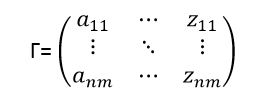
\includegraphics[scale=0.75]{grandematrice}%[height=70mm,width=70mm]
%\caption{\textbf{matrix of images database}}%
%\url {http://www.google.fr/}
\label{grandematrice}%
\end {center}
\end{figure} 
\\a:the subject 1 and z the subject n
\newpage
\item Step 4 : Calculate the average $\Psi$ of all images
\begin{figure}[bth]%[!ht]
\begin{center}
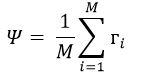
\includegraphics[scale=0.75]{moyenne}%[height=70mm,width=70mm]
%\caption{\textbf{average image}}%
%\url {http://www.google.fr/}
\label{moyenne}%
\end {center}
\end{figure} 
\item Step 5 : Substract the average image  from each image
\begin{figure}[bth]%[!ht]
\begin{center}
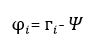
\includegraphics[scale=0.75]{centrage}%[height=70mm,width=70mm]
%\caption{\textbf{average image}}%
%\url {http://www.google.fr/}
\label{centrage}%
\end {center}
\end{figure}
\item Step 6 : Calculate the covariance matrix S
\begin{displaymath}
S= \sum_{i=1}^{M} \phi_{i} * \phi_{i} ^{T}= A * A ^{T} , A = (\phi_{1},\cdots \cdots  \cdots, \phi_{M})%\frac{1-q^{n+1}}{1-q}
\end{displaymath}

%\begin{figure}[bth]%[!ht]
%\begin{center}
%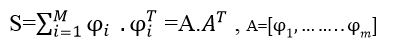
\includegraphics[scale=0.75]{cov_matrix}%[height=70mm,width=70mm]
%%\caption{\textbf{average image}}%
%%\url {http://www.google.fr/}
%\label{centrage}%
%\end {center}
%\end{figure}
\item Step 7 : After the covariance matrix ,eigenvalues and eigenvectors are computed.
Eigenvectors are then sorted by decreasing order.
%\begin{center}
%	\begin{tabular}{ll}
%	&\begin{math}
%		\sin \theta_{c} = n_{1}*\sin i_{c}\par \vspace{0.25cm}
%	\end{math}
%	\\

%{\color{red} \textbf{Formule de Snell-Descartes} :} & $n_{0}*\sin \theta_{c} = n_{1}*\sin i_{c}$ \\
%&  avec $n_{0} = 1$ (\emph{air})
%\end{tabular}
%\end{center}
\begin{center}
\begin{math}
   S * e_{i} =  \lambda_{i} * e_{i}
\end{math}


Formulas :
 $ \left\{\begin{array}{rl}
e_{i}= A * v_{i} & \mbox{eigenvectors } \\
\lambda_{i} = \mu_{i} & \mbox{eigenvalues
}\end{array}\right.$


\end{center}
  \end{itemize}
  
\subsection{Identification phase}  
The identification phase includes two steps and will help to recognize an input image in the image database.
 \begin{itemize}
 \item Step 1 : compute projection vectors
 
\begin{math}
   w_{k} = e^t_{k} * (\lambda_{i} -\psi)
\end{math} 
 
 
 

\paragraph{}
The projection vectors are called "weight vectors " and form a single matrix which will help for  compute  Euclidean distance. It also will help to find the class for an  input image.
\item Step 2 : compute the Euclidian distance
 
 \end {itemize}

This step in similar to the identification phase of Fisherfaces method.


 



%\begin{figure}[bth]%[!ht]
%\begin{center}
%\includegraphics[scale=0.75]{nom_image}%[height=70mm,width=70mm]
%\caption{\textbf{Titre image}}%
%\url {http://www.google.fr/}
%\label{label_image}%
%\end {center}
%\end{figure}

\clearpage
\section{Guide on Fisherfaces prototype}
This section is détailling differents steps on fisherfaces

\subsection{Learning phase}
The first part is also programmed into two steps the first step that is the learning phase is almost similar to fisherfaces' one. This similarity is onto the following common tasks:
\begin{itemize}
\item Loading of 10 images for every 40 subjects from the chosen database repertory;
\item Processing on images to get the mean image and center the images.

\end{itemize}

Once that common steps with eigenfaces are implemented or set up, we had to develop the LDA algorithm. This step can be describe as followed :
\paragraph{Calculation of the scatter matrices }
\begin{itemize}
\item Step 1 : We first get our $"y"$ list  gathering the numerotation of images according to the subject they belong to. Then this $"y"$ vector involved numbers from 0 to 39 since we have 40 subjects and each of this number are repeated ten times since every single subject has ten pictures. With the command $"c = np.unique(y)"$, we get the same vector in $"c"$ of numbers without them repeated tenth by sorting elements of $"y"$ and eliminating duplicates. Those numbers return the classes necessary to compute scatter matrix.
\item Step 2 : The second step will be to calculate the scatter matrices :

\begin{center}
	%\begin{tabular}{ll}
	 %&
		$Sw = Sw + np.dot((Xi-meanClass).T, (Xi-meanClass))$
		 Within classes scatter matrix (Sw)
	
	%{\color{red} \textbf{Within classes scatter matrix (Sw)} :}

\paragraph{}
%&  
$Sb = Sb + n * np.dot((meanClass - average).T, (meanClass - average))$
Between  classes scatter matrix (Sb)

%{\color{red} \textbf{Between  classes scatter matrix (Sb)} :} 
%\end{tabular}
\end{center}


\end{itemize} 
\paragraph{Calculation of fisherfaces }

\begin{itemize}
\item Step 3 :  We then apply the LDA algorithm to the previous reduced parameters
We need to find an optimal projection basis which both maximize the within dispersion relative to its matrix $Sw$ and minize the between dispersion relative to its matrix $Sb$.
\\
In other words, it consists in finding the "W" factor that maximize the Fisher optimizing Criteria :
%\begin{center}
%\begin{math}
%W= arg max_{T}(J(T))
%\end{math}
%\end{center}

\begin{center}
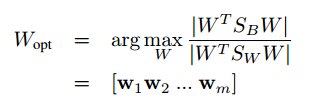
\includegraphics[scale=0.75]{critere_opt_fisher}%[critere_opt_fisher]
%\caption{\textbf{Titre image}}%
%\url {http://www.google.fr/}
%\label{label_image}%
\end {center}

\item Step 4 : We choose to use the PCA method to solve the problem we faced while trying to get W. The problem is about having matrices of different size. Then to resize them and be able to calculate W, PCA has been quite helful.



 
\end{itemize} 
\subsection{Identification phase}
The recognition of image from the basis obtained is similar to the previous method and take into consideration the calculation of distance such as euclidian distance, cosine \dots. We choose the euclidian distance.